\documentclass{beamer}
%
% Choose how your presentation looks.
%
% For more themes, color themes and font themes, see:
% http://deic.uab.es/~iblanes/beamer_gallery/index_by_theme.html
%
\mode<presentation>
{
  \usetheme{Boadilla}      % or try Darmstadt, Madrid, Warsaw, ...
  \usecolortheme{beaver} % or try albatross, beaver, crane, ...
  \usefonttheme{default}  % or try serif, structurebold, ...
  \setbeamertemplate{navigation symbols}{}
  \setbeamertemplate{caption}[numbered]
  
} 

\usepackage{xcolor,colortbl}
\usepackage[english]{babel}
\usepackage[utf8x]{inputenc}
\usepackage{courier}
\usepackage{dsfont}
\usepackage{verbatim} 
\usepackage{enumerate}
\usepackage{tikz}
\usepackage{multirow}
\usepackage{venndiagram}
\usepackage{epigraph} 
%\usepackage{xcolor}

%\usepackage{enumitem}

\usepackage{hyperref}
\hypersetup{
    colorlinks=true,
    linkcolor=blue,
    filecolor=magenta,      
    urlcolor=cyan,
}

% R stuff!
\usepackage{listings}
\definecolor{codegreen}{rgb}{0,0.6,0}
\definecolor{codegray}{rgb}{0.5,0.5,0.5}
\definecolor{codepurple}{rgb}{0.58,0,0.82}
\definecolor{backcolour}{rgb}{0.95,0.95,0.92}

\lstdefinestyle{mystyle}{
    backgroundcolor=\color{backcolour},    
    commentstyle=\color{codegreen},
    keywordstyle=\color{black},
    numberstyle=\tiny\color{codegray},
    stringstyle=\color{codepurple},
    basicstyle=\ttfamily\footnotesize,
    breakatwhitespace=false,         
    breaklines=true,                 
    captionpos=b,                    
    keepspaces=true,                 
    numbers=left,                    
    numbersep=5pt,                  
    showspaces=false,                
    showstringspaces=false,
    showtabs=false,                  
    tabsize=2
}

\lstset{style=mystyle}


\setbeamertemplate{enumerate items}[default]
\setbeamertemplate{itemize item}[triangle]

%\setitemize{label=\usebeamerfont*{itemize item}%
%  \usebeamercolor[fg]{itemize item}
%  \usebeamertemplate{itemize item}}



\title[SST-115 / STA-209]{Correlation}
\subtitle{Association between 2 Quantitative Variables}
\author{Grinnell College}
\date{September 23, 2024}

\graphicspath{{img/}}

\begin{document}

\begin{frame}
  \titlepage
\end{frame}



\begin{frame}{Outline}
On Friday we covered study design and how that affects the conclusions we make. These ideas will stick with us for the rest of the semester. \vspace{10mm}

What we will be covering today:\\
\vspace{3mm}
How to measure the strength of the relationship between quantitative variables.
\end{frame}



\begin{frame}{Review -- Z-scores}
A \textbf{z-score} or \textbf{standardized score} is a measurement that describes an observations \textit{value} relative to the mean and standard deviation of a group

\begin{align*}
z_i = \frac{x_i - \mu}{\sigma}
\end{align*}
\vspace{4mm}
In particular, there are two informative attributes related to a z-score:
\begin{enumerate}
\item The \textit{sign} of the z-score tells us if the observation is above or below the group mean
\item The \textit{magnitude} of the z-scores tells us how many standard deviations away from the mean an observation is
\end{enumerate}
\end{frame}



\begin{frame}{Review -- Scatterplots}
When we want to plot two quantitative variables $\rightarrow$ scatterplots
\begin{columns}
  \begin{column}{0.5\textwidth}
  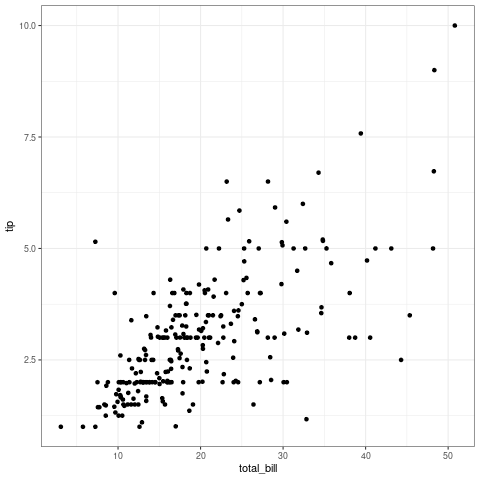
\includegraphics[scale=0.35]{img/scatter_tip.png}
  \end{column}
  \begin{column}{0.4\textwidth}
  Scatterplots let us see if there are \textit{associations} between quantitative variables
  \end{column}
\end{columns}
\end{frame}



\begin{frame}{Review -- Scatterplots}
Describing associations in scatterplots: \vspace{3mm}

\begin{itemize}
    \item \textbf{Form}: pattern? (linear / non-linear / curved / none)
    \item \textbf{Strength}: weak / moderate / strong
    \item \textbf{Direction}: positive / negative
    \item \textbf{Outliers}
\end{itemize}
\end{frame}


\begin{frame}{Extra on Outliers}
When we look for outliers in histograms and boxplots, it is fairly simple
\begin{itemize}
    \item boxplot $\rightarrow$ points outside the 'whiskers'
    \item histogram $\rightarrow$ gaps inbetween the bins
\end{itemize}
But! These do not always agree. We need to mention which we used to classify (i.e.: "...according to the histogram") \vspace{3mm}

\begin{columns}
 \begin{column}{0.45\textwidth}
    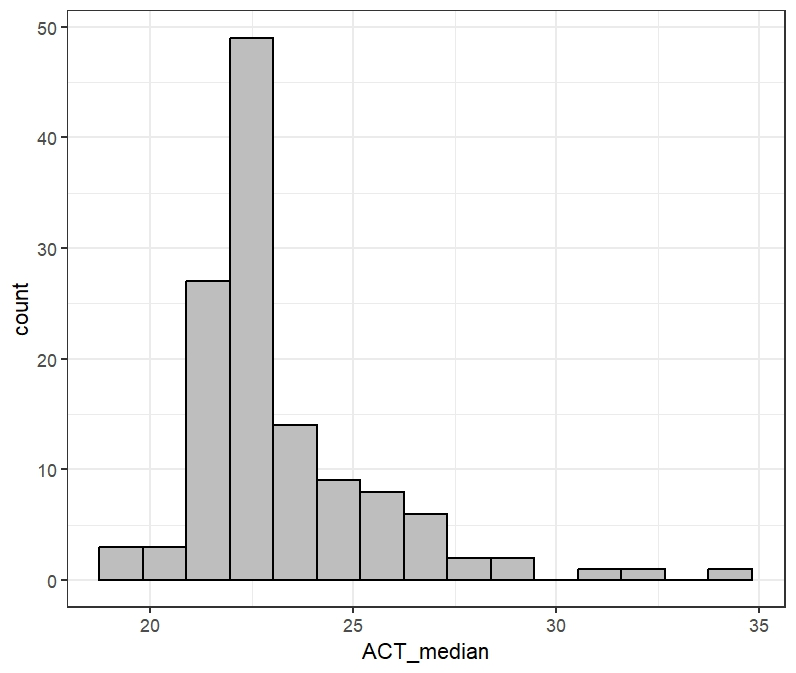
\includegraphics[scale=.38]{img/ACT_median_hist.jpeg}
 \end{column}
 \begin{column}{0.45\textwidth}
    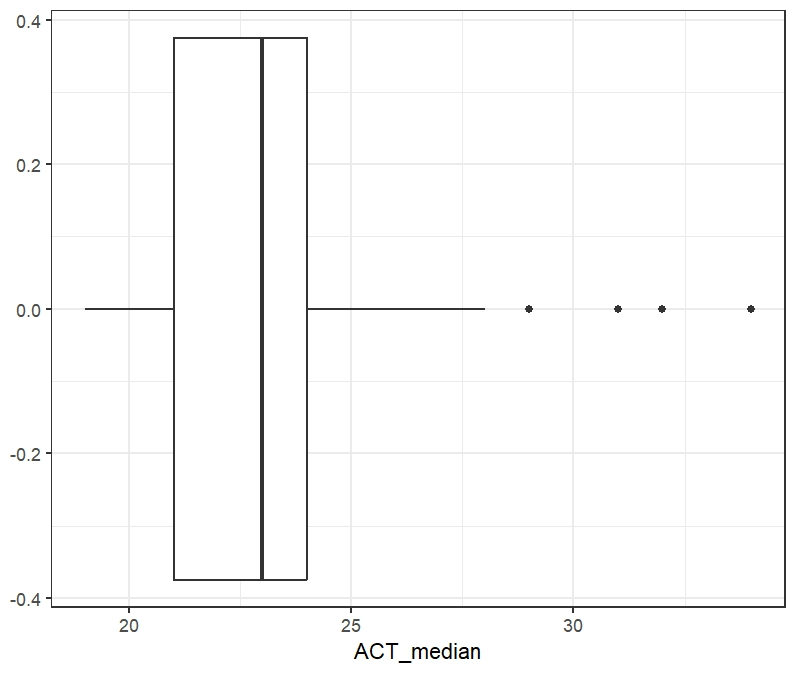
\includegraphics[scale=.38]{img/ACT_median_box.jpeg}
 \end{column}
\end{columns}
\end{frame}



\begin{frame}{Extra on Outliers}
\textbf{Outlier} in a scatterplot
\begin{itemize}
    \item very small or large values for one of the variables (or both!)
    \item does not follow the overall pattern
\end{itemize}

\begin{columns}
 \begin{column}{0.45\textwidth}
 \begin{center}
    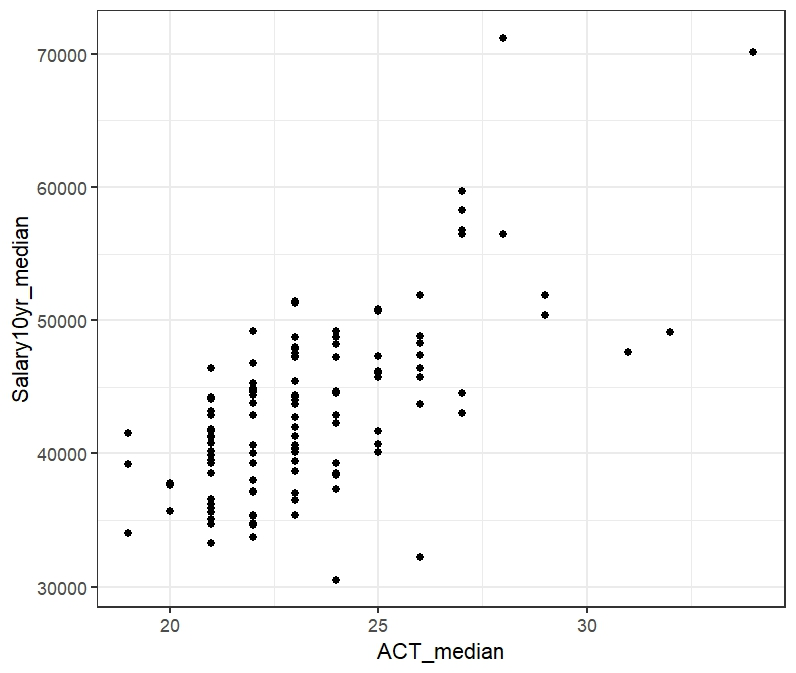
\includegraphics[scale=.4]{img/ACT_salary_scatter.jpeg}
    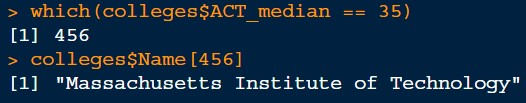
\includegraphics[scale=.5]{img/MIT_scatter_outlier.jpg}
\end{center}
 \end{column}
 \begin{column}{0.45\textwidth}
 \begin{center}
    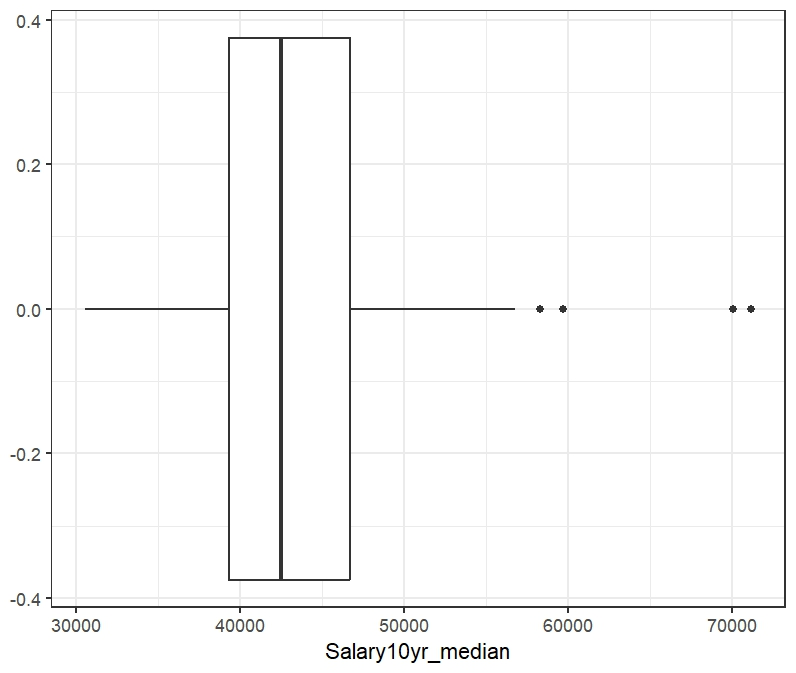
\includegraphics[scale=.25]{img/Salary_10yr_median_box.jpeg}
    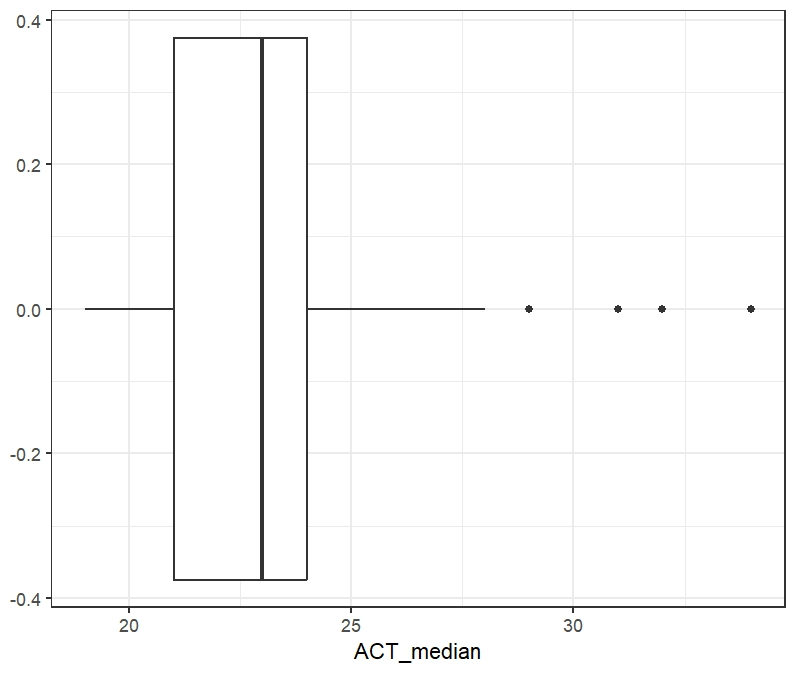
\includegraphics[scale=.25]{img/ACT_median_box.jpeg}
\end{center}
 \end{column}
\end{columns}
\end{frame}



\begin{frame}{Pearson's Height Data}
In the 1880's the Western scientific community was enthralled with the idea of quantifying heritable traits \vspace{2mm}

Karl Pearson collected data on the heights of 1,087 father's and their fully grown first born sons

\begin{table}[ht]
\centering
\begin{tabular}{rr}
  \hline
Father & Son \\ 
  \hline
65.0 & 59.8 \\ 
  63.3 & 63.2 \\ 
  65.0 & 63.3 \\ 
  65.8 & 62.8 \\ 
  61.1 & 64.3 \\ 
  63.0 & 64.2 \\  
  \vdots & \vdots \\
   \hline
\end{tabular}
\end{table}

\end{frame}

\begin{frame}{Height Data}
\begin{center}
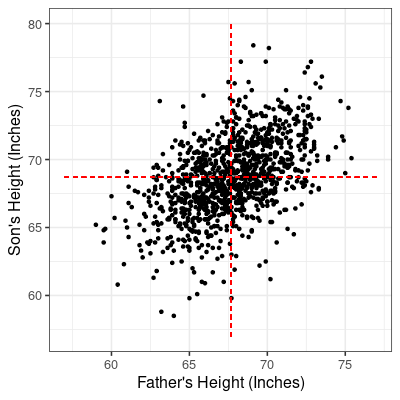
\includegraphics[scale=0.5]{father_son.png}
\end{center}
\end{frame}

\begin{frame}{Pearson's Correlation Coefficient}
Heights clearly associated, but how to quantify? \vspace{2mm}

Building upon the work from French scientist Francis Galton, Pearson developed the \textbf{Pearson's correlation coefficient (r)}:
\vspace{2mm}
\begin{align*}
r &= \frac{1}{n-1} \sum_{i=1}^n \left( \frac{x_i - \overline{x}}{s_x} \right) \left( \frac{y_i - \overline{y}}{s_y} \right) \\
&= \frac{1}{n-1} \sum_{i=1}^n (z_{x_i} ) (z_{y_i})
\end{align*}
\vspace{2mm}

If above-average values of $X$ are common among cases with above-average values of $Y$ (or vice-versa), we should expect $r$ to be positive
\end{frame}

\begin{frame}{Height Data -- Standardized}
\begin{center}
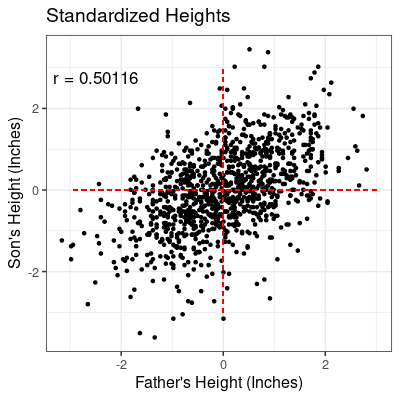
\includegraphics[scale=0.5]{father_son2.png}
\end{center}
\end{frame}

\begin{frame}{Correlation Examples}
Pearson's correlation coefficient tells us the strength of \textit{linear} association between two quantitative variables (and direction!) 

\begin{center}
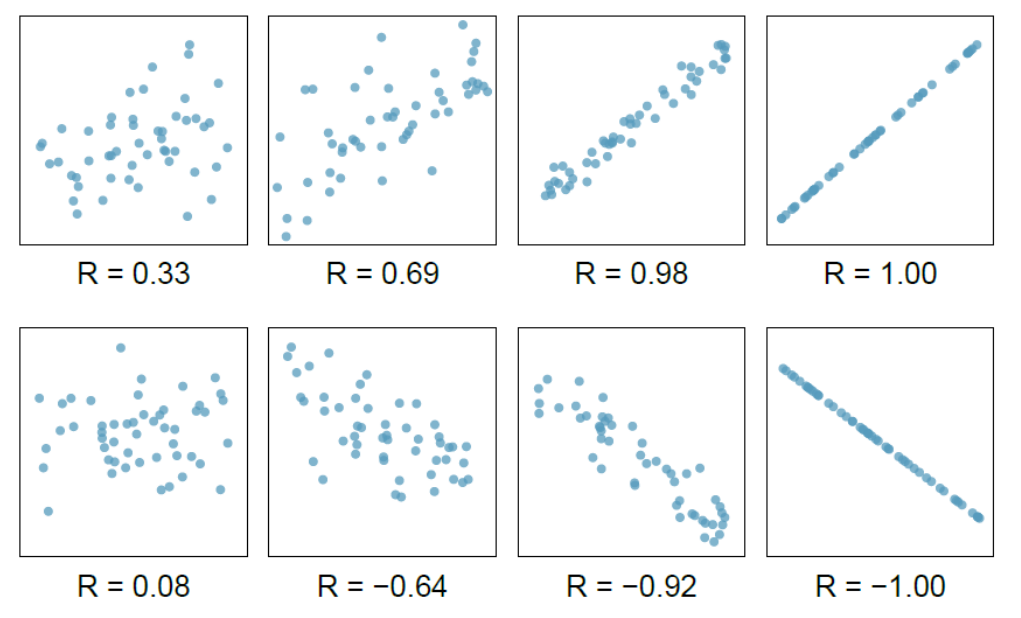
\includegraphics[scale=0.25]{cor_examples.png}
\end{center}
\end{frame}

\begin{frame}{What is considered ``strong"?}
\begin{center}
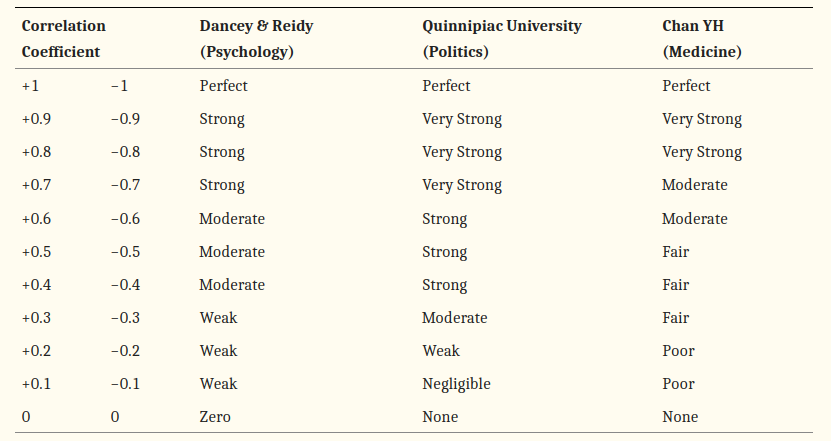
\includegraphics[scale=0.4]{correlation_table.png}
\end{center}
{\tiny Source: https://www.ncbi.nlm.nih.gov/pmc/articles/PMC6107969/}
\end{frame}

\begin{frame}{Correlation Examples}
\begin{center}
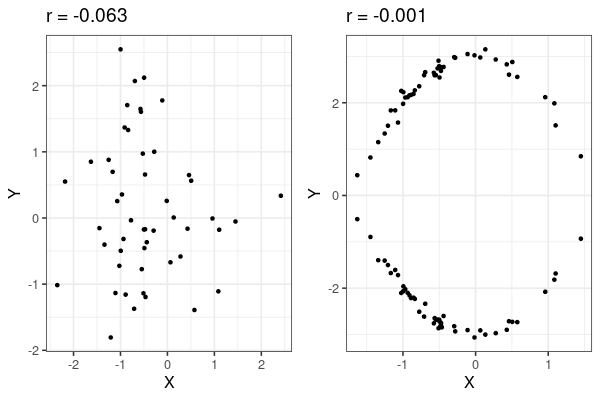
\includegraphics[scale=0.5]{no_corr_example.png}
\end{center}
\end{frame}

\begin{frame}{Correlation Properties}
\textbf{Properties:}
\begin{itemize}
    \item r has no units
    \item r measures the strength of a linear relationship
    \item r is between -1 and 1
    \item The closer r is to 0 $\rightarrow$ weaker relationship
    \item The further r is from 0 $\rightarrow$ stronger relationship
    \item r=0 $\rightarrow$ no linear relationship
    \item changing scale of either variable doesn't affect r value
\end{itemize}
\end{frame}

\begin{frame}{Pitfalls}
If we get a value for r close to +1 or -1, it does \textbf{not} mean the relationship actually is linear (double-check the scatterplot!)
\begin{center}
    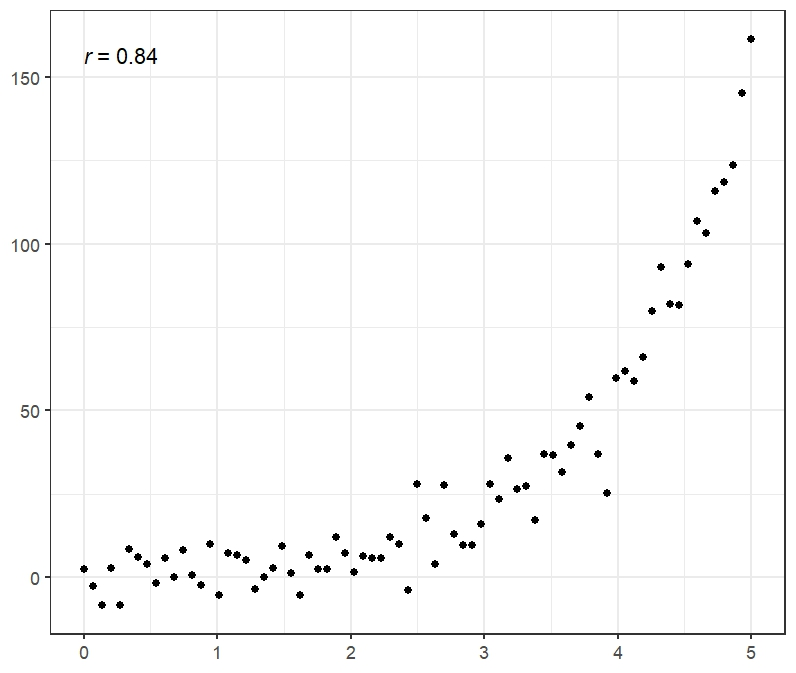
\includegraphics[scale=.55]{img/nonlinear_corr_ex.jpeg}
\end{center}
\end{frame}



\begin{frame}{Non-linear Association}
In addition to Pearson, we have \textbf{Spearman's rank correlation} (denoted $\rho$) where the values of $X$ and $Y$ are replaced with their rank order from smallest to largest before correlating:
$$
\begin{aligned}
X &= \{2,4,6,9,8 \} \\
Y &= \{7,4,1,5,3 \} 
\end{aligned}
 \quad
 \Longrightarrow
 \quad
\begin{aligned}
X_{rank} &= \{1,2,3,5,4 \} \\
Y_{rank} &= \{5,3,1,4, 2\} 
\end{aligned}
$$

\vspace{4mm}

Whereas Pearson's $r$ measures \textit{linear association}, Spearman's $\rho$ measures the \textit{monotonic association} (increasing or decreasing)

\end{frame}

\begin{frame}{Non-linear Assocation}
\begin{align*}
y = x^3
\end{align*}
\begin{center}
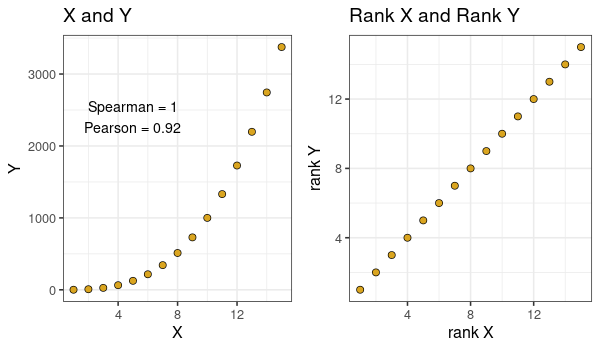
\includegraphics[scale=0.5]{cubic_actually.png}
\end{center}
\end{frame}

\begin{frame}{Spearman Correlation}
Spearman's correlation is more robust to outliers
\begin{center}
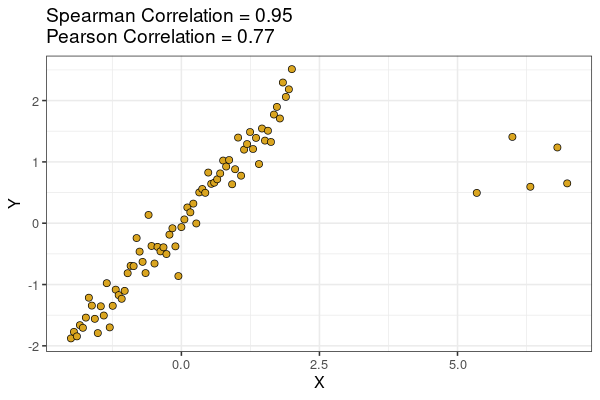
\includegraphics[scale=0.5]{outliers.png}
\end{center}
\end{frame}

\begin{frame}{``Datasauraus Dozen"}
\begin{center}
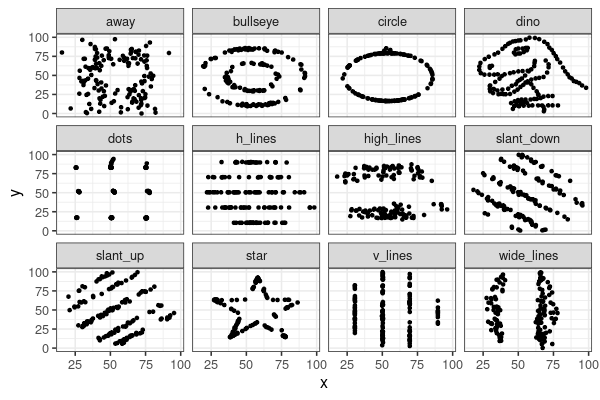
\includegraphics[scale=0.5]{dozen.png}
\end{center}
\end{frame}


\begin{frame}{Ecological Correlation}
\textbf{Ecological correlations} compare variables for data that have been aggregated at an ecological level \\ \vspace{2mm}

\begin{itemize}
\item Countries
\item States
\item Schools
\end{itemize}
\vspace{4mm}
The \textit{ecological fallacy} is a fallacy in which a conclusion is drawn that, because a correlation exists at a group level, it must exist at the individual level as well

\end{frame}


\begin{frame}{College Ecological Fallacy}

Grouping by region, the correlation between (mean) admission rate and (mean) median debt is $r = -0.66$
\begin{center}
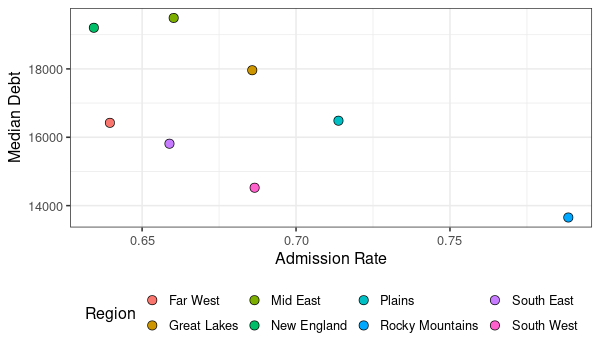
\includegraphics[scale=0.5]{cc_group.png}
\end{center}
\end{frame}

\begin{frame}{College Ecological Fallacy}
\footnotesize
This completely disappears when we remove consideration of region, with $r = 0.02$
\begin{center}
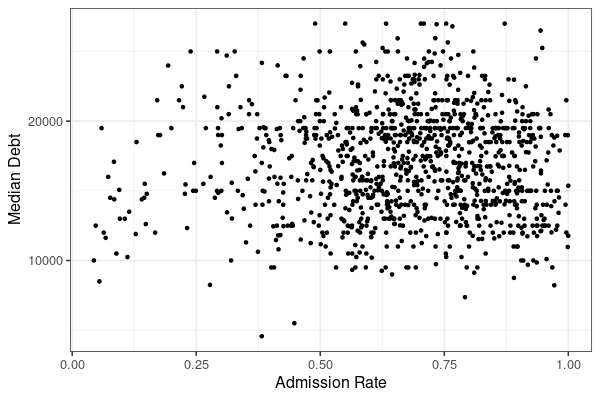
\includegraphics[scale=0.5]{cc_all.png}
\end{center}
\end{frame}

\begin{frame}{College Ecological Fallacy}

\begin{center}
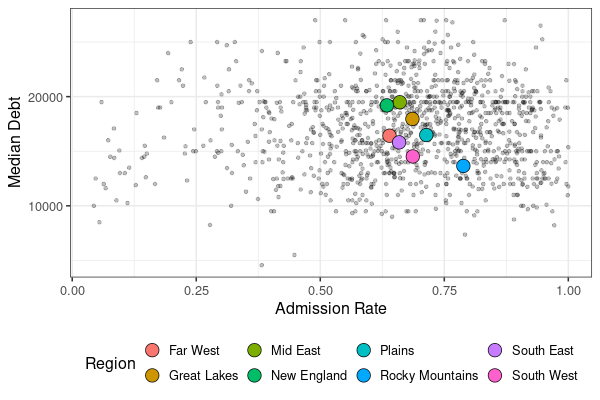
\includegraphics[scale=0.5]{cc_all2.png}
\end{center}
\end{frame}

\begin{frame}{Correlation $\neq$ Causation}
    We can have a large correlation value between 2 variables. This does not mean the explanatory variable is \textit{causing} a change in the response variable. \vspace{4mm}

Examples with high correlation but where no causal claims can be made:
\begin{itemize}
    \item Literacy Rate and Gross Domestic Product (GDP) in countries
    \item average number of TVs in a household and Life expectancy of countries
    \item ice-cream sales and shark attacks
\end{itemize} \vspace{6mm}

\textbf{Lurking Variable}: a third variable that explains the relationship between two variables with high correlation
\end{frame}



\begin{frame}{Review}

\begin{itemize}
\item \textbf{Pearson's correlation} strength of \textit{linear association} (and direction)
\begin{itemize}
\item Correlation is \textit{average product of z-scores}
\end{itemize}
\item \textbf{Spearman  rank correlation} useful for data with outlier's or non-linear (but monotone) relationship
\item Be careful with \textbf{ecological correlations} -- inference for a group is not always valid for individuals
\item Correlation $\neq$ Causation
\end{itemize}


\end{frame}




%
%
%\begin{frame}{Pearson's Correlation Coefficient}
%
%\end{frame}
%
%
%\begin{frame}{correlation}
%see its just this
%\end{frame}




%%%%%%%%%%%%%%%%

%\begin{frame}
%\begin{columns}
%
%  \begin{column}{0.45\textwidth}
%%
%  \end{column}
%  \begin{column}{0.45\textwidth}
%%
%  \end{column}
%
%\end{columns}
%\end{frame}


\end{document}
